La inicialización del sistema cuenta de varias partes:
\begin{itemize}
    \item Configuración del microcontrolador.
    \item Deshabilitar las interrupciones.
    \item Inicializar el reloj.
    \item Inicializar los pines y los puertos.
    \item Inicializar el módulo \ac{PWM}.
    \item Inicializar el módulo \ac{UART}.
    \item Establecer el modo de operación del \texttt{CORCON}.
    \item Habilitar de nuevo las interrupciones.
\end{itemize}

Toda esta lógica se aúna en la función \texttt{system\_initialize}:

\lstinputlisting[linerange={359-367}, firstnumber=359, caption=, style=C]{pArm-S2/pArm.X/init.c}

\subsubsection{Configuración del microcontrolador}
La configuración del microcontrolador es una parte crucial a la hora de poder
trabajar con el dispositivo ya que permite definir cómo se va a comportar ante
ciertas situaciones.

La configuración se realiza mediante una serie de \texttt{pragmas} que definen
tanto qué opciones están habilitadas como el modo de funcionamiento de ciertos
componentes.

De todas las configuraciones establecidas, destacan las siguientes:

\begin{itemize}
    \item \lstinline[style=C]{#pragma config PLLKEN = ON} -- habilita el bit de bloqueo
    del \texttt{PLL} que permite saber cuándo un cambio en la frecuencia del oscilador
    es efectivo.
    \item \lstinline[style=C]{#pragma config IOL1WAY = OFF} -- permite cambiar el modo
    de funcionamiento de los periféricos más de una única vez.
    \item \lstinline[style=C]{#pragma config FCKSM = CSECME} -- permite cambiar la
    frecuencia del reloj y habilita el \textit{Fail--Safe Clock Monitor}.
    \item \lstinline[style=C]{#pragma config PWMLOCK = OFF} -- permite que un puerto
    \ac{PWM} pueda ser utilizado para otros propósitos, como puede ser para la \ac{UART}.
\end{itemize}

La lista completa de pragmas se define en el fichero \texttt{pragmas.h} (listado de
código \ref{lst:pragmas_h}).

\subsubsection{Inicialización del reloj del sistema}
La rutina de inicialización del reloj define la frecuencia a la que va a trabajar
el sistema. Para este proyecto se cuenta con una frecuencia inicial de oscilación
$F_{OSC} = \numprint[MHz]{7.3728}$ y se busca alcanzar una nueva frecuencia de
oscilación $F_{OSC}' \approx \numprint[MHz]{120}$.

Según el manual del fabricante, la frecuencia máxima a la que podría trabajar
el microcontrolador dsPIC33E sería de $\numprint[MHz]{140}$ con una temperatura
máxima de $\numprint[\celsius]{85}$ \cite{microchipDsPIC33EPIC24EFRM2012}. Para
evitar alcanzar ese margen y que sea necesario utilizar un disipador, se establece 
la frecuencia $\numprint[MHz]{20}$ por debajo de la máxima.

El cálculo de la nueva frecuencia de oscilación responde a la ecuación \ref{eq:fosc}
provista por el manual \cite{microchipDsPIC33EPIC24EFRM2012}:

\begin{equation}\label{eq:fosc}
    F_{OSC} = F_{IN} \cdot \frac{M}{N_1 + N_2} = F_{IN} \cdot \frac{PLLDIV + 2}{\left(PLLPRE + 2\right) \cdot 2\left(PLLPOST + 1\right)}
\end{equation}

donde

\begin{equation*}
    \left\{
        \begin{aligned}
            N_1 &= PLLPRE + 2 \\
            N_2 &= 2 \cdot \left(PLLPOST + 1\right) \\
            M &= PLLDIV + 2
        \end{aligned}
    \right.
\end{equation*}

En particular, se puede conseguir una frecuencia de oscilación de $\numprint[MHz]{119.808}$
estableciendo los siguientes valores de $N_1$, $N_2$ y $M$ (ecuación \ref{eq:fosc_final}):

\begin{equation}\label{eq:fosc_final}
    \begin{gathered}  
        F_{OSC} = \numprint[MHz]{7.3728} \cdot \frac{65}{2 \cdot 2} = \numprint[MHz]{119.808}, \\[2ex]
        \left\{
            \begin{aligned}
                N_1 &= 2 \\
                N_2 &= 2 \\
                M &= 65
            \end{aligned}
        \right.
    \end{gathered}
\end{equation}

De esta manera, se introducen en los registros \texttt{PLLPRE}, \texttt{PLLPOST} y
\texttt{PLLDIV} los valores $0$, $0$ y $63$ respectivamente. Una vez cambiados los
registros se espera de forma activa a que cambie la frecuencia del reloj
(\texttt{OSWEN = 0} y \texttt{LOCK = 1}).

Esta lógica se encuentra en la función \texttt{init\_clock}:
\lstinputlisting[linerange={34-77}, firstnumber=34, caption=, style=C]{pArm-S2/pArm.X/init.c}

\subsubsection{Inicialización de los pines y puertos}
En el dsPIC33E se utilizan múltiples pines y puertos que han de ser inicializados para
el control de distintos periféricos. Los distintos pines y puertos del microcontrolador
se muestran en la figura \ref{fig:dspic33e_upper}:

\begin{figure}[H]
    \centering
    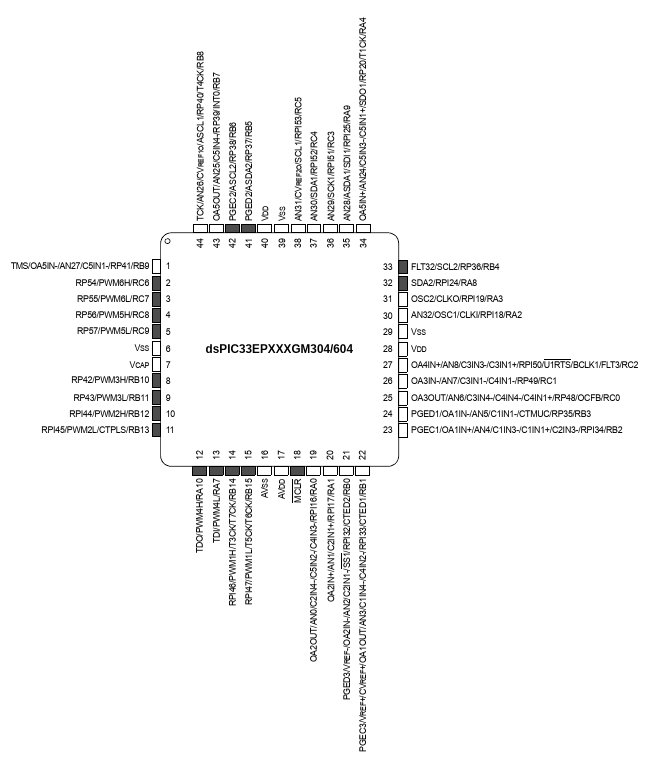
\includegraphics[width=\linewidth]{pictures/dspic33e_upper.png}
    \caption{Vista esquemática del dsPIC33E \cite{datasheet.ex7759009FCCCDatasheetHoja}.}
    \label{fig:dspic33e_upper}
\end{figure}

En particular, se utilizan los pines 41 -- 44 para controlar los LEDs colocados en la
placa, los pines 19 -- 22 para controlar los microinterruptores conectados que actúan
como fin de carrera. Esto se encuentra en la función \texttt{init\_ports}:

\lstinputlisting[linerange={326-357}, firstnumber=326, caption=, style=C]{pArm-S2/pArm.X/init.c}

Por otro lado, se utilizan los pines 9, 11, 13 y 15 para controlar la señal \ac{PWM}
que controla los motores. Esto se realiza en la función \texttt{initPWM}:

\lstinputlisting[linerange={158-161}, firstnumber=158, caption=, style=C]{pArm-S2/pArm.X/init.c}

Finalmente, para controlar la \ac{UART} se utilizan los pines 3 y 2, los cuales son
remapeables y es necesario establecer a qué puerto va cada uno y qué funcionalidad cumple.

Esto se realiza en la función \texttt{initUART}:
\lstinputlisting[linerange={87-91}, firstnumber=87, caption=, style=C]{pArm-S2/pArm.X/init.c}

\subsubsection{Inicialización del módulo \ac{PWM}}
El módulo \ac{PWM} requiere de una inicialización propia para establecer la frecuencia
de funcionamiento del mismo. Los motores que se están utilizando son servomotores
y se controlan mediante una señal de pulsos cada cierto tiempo, establecido por el 
diseño del fabricante.

Para el servomotor Parallax 900-00005, se requiere un periodo de $\numprint[ms]{20}$
(imagen \ref{fig:servo_pwm}):

\begin{figure}[H]
    \centering
    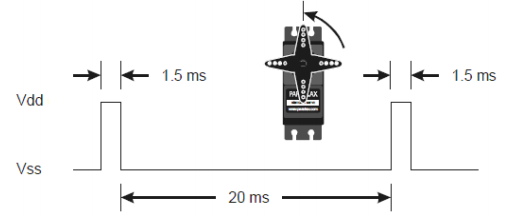
\includegraphics[width=.6\linewidth]{pictures/servo_pwm.png}
    \caption{Periodo de la señal \ac{PWM} que ha de ser enviada al servomotor \cite{rs-online90000005ServomotorParallax}.}
    \label{fig:servo_pwm}
\end{figure}

En el dsPIC33E, el módulo \ac{PWM} se configura estableciendo un valor en el registro
\texttt{PTPER}, el cual respeta la siguiente ecuación (ecuación \ref{eq:ptper}):

\begin{equation}\label{eq:ptper}
    PTPER = \frac{F_{OSC}}{F_{PWM} \cdot PWM_{Prescaler}}
\end{equation}

El registro \texttt{PTPER} es un registro de 16 bits, por lo que el valor más alto
que puede contener es $\numprint{65536}$. Si el valor supera el máximo de dicho registro,
se habrá de incrementar el prescalado para poder reducirlo. Según el manual \cite{microchipDsPIC33EPIC24EFamily2011},
se encuentran disponibles prescalados desde $2^0$ hasta $2^6$ (incrementándose en
potencias de dos).

De esta manera, para controlar los servomotores, se tiene que:

\begin{equation*}
    \left\{
        \begin{aligned}
            F_{PWM} &= T_{PWM}^{-1} = \frac{1}{20} = \numprint[Hz]{50} \\
            F_{OSC} &= \numprint[MHz]{119.808} \\
            PWM_{Prescaler} &= 1:2^5 = 1:32 \equiv Prescaler=101
        \end{aligned}
    \right.
\end{equation*}

por lo que el valor a introducir en el registro \texttt{PTPER} es (ecuación \ref{eq:ptper_res}):
\begin{equation}\label{eq:ptper_res}
    PTPER = \frac{\numprint[MHz]{119.808}}{\numprint[Hz]{50} \cdot 32} = \numprint{37440}
\end{equation}

Finalmente, se configuran los módulos \ac{PWM} para trabajar en modo verdaderamente
independiente. Esto es, se cuenta con dos señales \ac{PWM}: \texttt{PWMxL} y \texttt{PWMxH},
que pueden funcionar en modo combinado de 16 bits, pero para tener más posibilidades
se configuran ambas señales como señales independientes, esto es, funcionan sin alterar
la salida que se produce en la otra.

Todo el código de inicialización se encuentra en la función \texttt{initPWM}:

\lstinputlisting[linerange={157-251}, firstnumber=157, caption=, style=C]{pArm-S2/pArm.X/init.c}

\subsubsection{Inicialización de la \ac{UART}}
El módulo \ac{UART} permite la comunicación entre los dos sistemas \ac{S1} y \ac{S2}.
En el proceso de diseño se estableció la tasa de transmisión en $\numprint[baud]{9600}$,
por lo que se ha de configurar el dsPIC33E para que funcione a esta velocidad.

Según el manual del microcontrolador, el valor del \textit{baudrate} se ha de establecer
en el registro \texttt{UxBRG} y responde a la siguiente ecuación (ecuación \ref{eq:brg}):

\begin{equation}\label{eq:brg}
    UxBRG = \frac{F_{CY}}{16 \cdot Baud~rate} - 1
\end{equation}

Según la configuración establecida anteriormente, se sabe que la frecuencia del ciclo
de instrucción ($F_{CY}$) es:

\begin{equation*}
    F_{CY} = \frac{F_{OSC}}{2} = \frac{\numprint[MHz]{119.808}}{2} = \numprint[MHz]{59.904}
\end{equation*}

por lo que se tiene que el valor del registro \texttt{UxBRG} es (ecuación \ref{eq:brg_res}):

\begin{equation}\label{eq:brg_res}
    UxBRG = \frac{\numprint[MHz]{59.904}}{16 \cdot 9600} - 1 = 389
\end{equation}

Por otra parte, se configuran múltiples parámetros de la \ac{UART} para:

\begin{itemize}
    \item Producir una interrupción en cada caracter recibido por $R_X$.
    \item El estado de inactividad no se invierta, esto es, tenga un nivel alto.
    \item Se utiliza el modo de velocidad estándar de la \ac{UART}.
    \item Las transmisiones son de 8 bits sin bit de paridad.
    \item La transmisión de bits así como su recepción generan una interrupción.
\end{itemize}

Todo esto se encuentra definido en la función \texttt{initUART}:

\lstinputlisting[linerange={79-155}, firstnumber=79, caption=, style=C]{pArm-S2/pArm.X/init.c}
